\documentclass[shownotes,11pt, aspectratio=169]{beamer}

\usepackage{pgfpages}
% These slides also contain speaker notes. You can print just the slides,
% just the notes, or both, depending on the setting below. Comment out the want
% you want.
\setbeameroption{hide notes} % Only slide
%\setbeameroption{show only notes} % Only notes
%\setbeameroption{show notes on second screen=right} % Both
\AtBeginSection[]{
  \begin{frame}
  \vfill
  \centering
  \begin{beamercolorbox}[sep=8pt,center,shadow=true,rounded=true]{title}
    \usebeamerfont{title}\insertsectionhead\par%
  \end{beamercolorbox}
  \vfill
  \end{frame}
}


\usepackage{helvet}
\usepackage[default]{Fira Sans}
\usepackage{array}
\usepackage{caption}
%\usepackage[clean]{svg}
\usepackage{tikz}
\usepackage{verbatim}
\setbeamertemplate{note page}{\pagecolor{yellow!5}\insertnote}
\usetikzlibrary{positioning}
\usetikzlibrary{snakes}
\usetikzlibrary{calc}
\usetikzlibrary{arrows}
\usetikzlibrary{decorations.markings}
\usetikzlibrary{shapes.misc}
\usetikzlibrary{matrix,shapes,arrows,fit,tikzmark}
\usepackage{amsmath}
\usepackage{mathpazo}
\usepackage{hyperref}
\usepackage{lipsum}
\usepackage{multimedia}
\usepackage{graphicx}
\usepackage{multirow}
%\usepackage{graphicx}
\usepackage{dcolumn}
\usepackage{bbm}
\usepackage{tfrupee}

%%%%more packages%%%
\usepackage{tabulary}
%\usepackage[usenames,dvipsnames]{pstricks}
%\usepackage[capposition=top]{floatrow}
\usepackage{lineno,hyperref}
\usepackage{epsfig}
\usepackage{graphics}
\usepackage{psfrag}
\usepackage{etoolbox}
\appto\TPTnoteSettings{\footnotesize}
\usepackage{color}
\usepackage{amsfonts}
\usepackage{amsmath}
\usepackage{mathrsfs}
\usepackage{eucal}
\usepackage{amsbsy}
\usepackage{url}
\usepackage{color}
\usepackage{lineno}
\usepackage{amssymb}
%\usepackage{adjustbox}
\newcommand{\overbar}[1]{\mkern 2.5mu\overline{\mkern-2.5mu#1\mkern-2.5mu}\mkern 2.5mu}
\usepackage{booktabs} %%To use toprule, midrule, bottomrule, etc.
\usepackage{rotating} %% To use sidewaystable 
\usepackage{dcolumn}
\usepackage{longtable}
\usepackage{threeparttable}
\usepackage{tabularx}
%%%%

\newcolumntype{d}[0]{D{.}{.}{5}}

\usepackage{changepage}
\usepackage{appendixnumberbeamer}
\newcommand{\beginbackup}{
   \newcounter{framenumbervorappendix}
   \setcounter{framenumbervorappendix}{\value{framenumber}}
   \setbeamertemplate{footline}
   {
     \leavevmode%
     \hline
     box{%
       \begin{beamercolorbox}[wd=\paperwidth,ht=2.25ex,dp=1ex,right]{footlinecolor}%
%         \insertframenumber  \hspace*{2ex} 
       \end{beamercolorbox}}%
     \vskip0pt%
   }
 }
\newcommand{\backupend}{
   \addtocounter{framenumbervorappendix}{-\value{framenumber}}
   \addtocounter{framenumber}{\value{framenumbervorappendix}} 
}


\usepackage{graphicx}
\usepackage[space]{grffile}

% These are my colors -- there are many like them, but these ones are mine.
\definecolor{blue}{RGB}{0,114,178}
\definecolor{red}{RGB}{213,94,0}
\definecolor{yellow}{RGB}{240,228,66}
\definecolor{green}{RGB}{0,158,115}
\definecolor{applegreen}{rgb}{0.55, 0.71, 0.0}
\definecolor{ao(english)}{rgb}{0.0, 0.5, 0.0}

\hypersetup{
  colorlinks=false,
  bookmarks=true,
  linkbordercolor = {white},
  linkcolor = {blue}
}


%% I use a beige off white for my background
\definecolor{MyBackground}{RGB}{255,253,218}

%% Uncomment this if you want to change the background color to something else
\setbeamercolor{background canvas}{bg=MyBackground}

%% Change the bg color to adjust your transition slide background color!
\newenvironment{transitionframe}{
  \setbeamercolor{background canvas}{bg=yellow}
  \begin{frame}}{
    \end{frame}
}

\setbeamercolor{frametitle}{fg=blue}
\setbeamercolor{title}{fg=black}
\setbeamertemplate{footline}[frame number]
\setbeamertemplate{navigation symbols}{} 
\setbeamertemplate{itemize items}{-}
\setbeamercolor{itemize item}{fg=blue}
\setbeamercolor{itemize subitem}{fg=blue}
\setbeamercolor{enumerate item}{fg=blue}
\setbeamercolor{enumerate subitem}{fg=blue}
\setbeamercolor{button}{bg=MyBackground,fg=blue,}



% If you like road maps, rather than having clutter at the top, have a roadmap show up at the end of each section 
% (and after your introduction)
% Uncomment this is if you want the roadmap!
% \AtBeginSection[]
% {
%    \begin{frame}
%        \frametitle{Roadmap of Talk}
%        \tableofcontents[currentsection]
%    \end{frame}
% }
\setbeamercolor{section in toc}{fg=blue}
\setbeamercolor{subsection in toc}{fg=red}
\setbeamersize{text margin left=1em,text margin right=1em} 

\newenvironment{wideitemize}{\itemize\addtolength{\itemsep}{10pt}}{\enditemize}

\title[]{\textcolor{blue}{Macroeconomics: Lecture 9}}
\author[SM]{Sumit Mishra}
\institute[IFMR]{\small{\begin{tabular}{c}
IFMR, Sri City \\
\end{tabular}}}

\date{31 October, 2019}

%\documentclass[10pt]{beamer}
%\input{slideclass.tex}







%----------------------------------------------------------------------------------------
%	TITLE PAGE
%----------------------------------------------------------------------------------------


\begin{document}



%----------------------------------------------------------------------------------------
%	PRESENTATION SLIDES
%----------------------------------------------------------------------------------------
\begin{frame}{Agenda}
\begin{itemize}
\item The distinction between the \textit{real} and the \textit{nominal} interest rate.
\item The role of expectations in financial markets.
\item The role of expectations in consumption and investment decisions. 
\item Material: Blanchard, Chapters 14, 15, and 16.
\end{itemize}
\end{frame}

\section{Chapter 14}
\begin{frame}{Nominal Vs Real Interest Rate}
The real interest rate is equal to the nominal interest rate minus the expected inflation.
\begin{equation*}
r_t = i_t - \pi_{t+1}^e
\end{equation*}
\end{frame}

\begin{frame}
\begin{center}
%\begin{figure}[ht]
\centering
 \makebox[\linewidth][c]{
  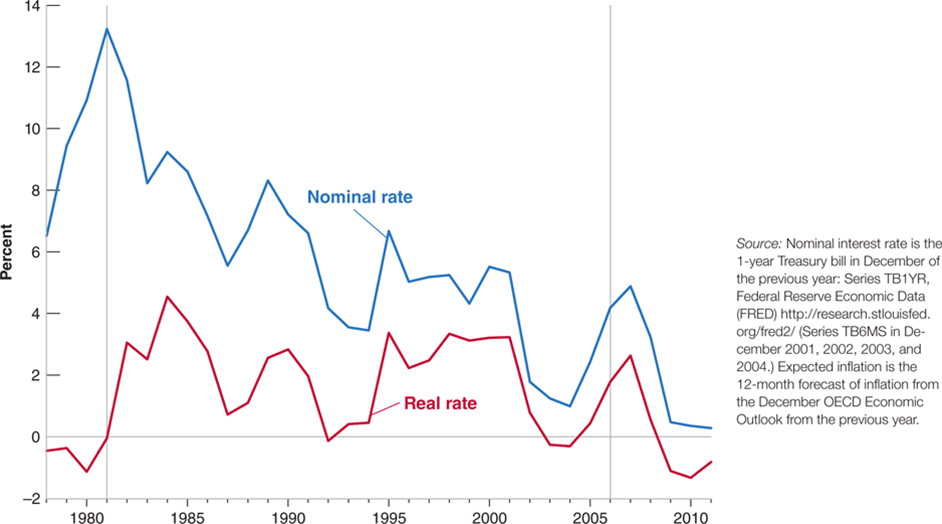
\includegraphics[scale=0.55]{graphs/L9F1.png}}
%\caption*{Welcome to \textcolor{ao(english)}{impact evaluation methods for business decisions}}
%\end{figure}
\end{center}
\begin{itemize}
\item Nominal rate might be low, but we need to look at the real rate to check for economy's health.
\pause
\item Aren't low rates and low inflation good for economy?
\end{itemize}
\end{frame}

\begin{frame}{Why Deflation Can Be Devastating}
\makebox[\linewidth][c]{
  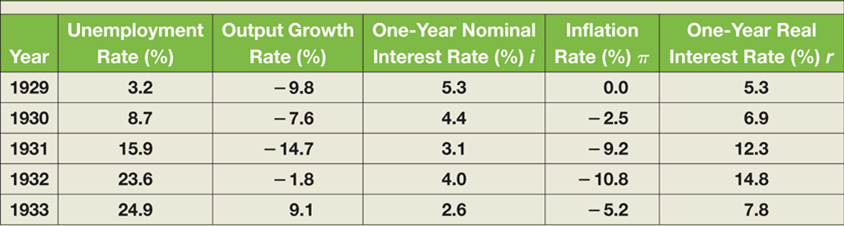
\includegraphics[scale=0.55]{graphs/L9F2}}
\begin{itemize}
\item In 1933, the US economy was stuck in a \textbf{deflation trap}.
\item Among other things, rising real rates led to worsening of the situation.
\end{itemize}
\end{frame}

\begin{frame}{The $IS-LM$ Model Revisited}
\begin{itemize}
\item Investments and consumption are determined by the \textbf{real interest rates}.
\item The rate that the RBI announces is the \textbf{nominal interest rate}.
\item Therefore, the impact of monetary policy on output \pause depends upon how nominal rates affect real rates.
\end{itemize}
\end{frame}

\begin{frame}{Money Growth, Inflation, and Interest Rate}
Two key features: real or nominal; short or long run.
\begin{itemize}
\item[1] \textbf{SR:} $\uparrow$\texttt{Money Growth} $\Rightarrow$ $\downarrow$\texttt{Nominal Interest Rate} \pause
\item[2] \textbf{MR:} $\uparrow$\texttt{Money Growth} $\Rightarrow$ $\uparrow$\texttt{Nominal Interest Rate} \pause
\item[3] \textbf{SR:} $\uparrow$\texttt{Money Growth} $\Rightarrow$ $\downarrow$\texttt{Real Interest Rate} \pause
\item[4] \textbf{MR:} $\uparrow$\texttt{Money Growth} $\Rightarrow$ $\leftrightarrow$\texttt{Real Interest Rate}
\end{itemize}
\end{frame}

\begin{frame}{The Short Run}
\begin{itemize}
\item The feature of the model is: \pause \textcolor{ao(english)}{prices do not adjust quickly}.
\item People and firms do not revise their inflation expectations immediately.
\item So, short-run monetary policy story is a happy story.
\end{itemize}
\end{frame}

\begin{frame}{The Medium Run}
\textit{The rate of inflation = the rate of money growth}
\begin{itemize}
\item Everything in the medium run is benchmarked against the ``natural'' value.
\pause
\item We also know that 
      \[ i = r + \pi^e \]
\item Because inflation is equal to money growth, we get:
     \[ i = r + g_M \]
\pause
\item A 5\% increase in money growth leads to a 5\% rise in inflation and a 5\% rise in nominal rates.
\item This is known as the \textbf{Fisher hypothesis}.
\end{itemize}
\end{frame}

\begin{frame}{The Short Run to the Medium Run}
\begin{columns}[T] % align columns
\begin{column}{.36\textwidth}
\begin{itemize}
\item $\downarrow$\texttt{Interest Rate} $\Rightarrow$ $\uparrow$\texttt{Output}
\pause
\item Over time: inflationary pressure sets in. 
\pause
\item Real money stock goes down.
\pause
\item $\uparrow$\texttt{Interest Rate}.
\end{itemize}
\end{column}
\hfill
\pause
\begin{column}{.54\textwidth}
\makebox[\linewidth][c]{
  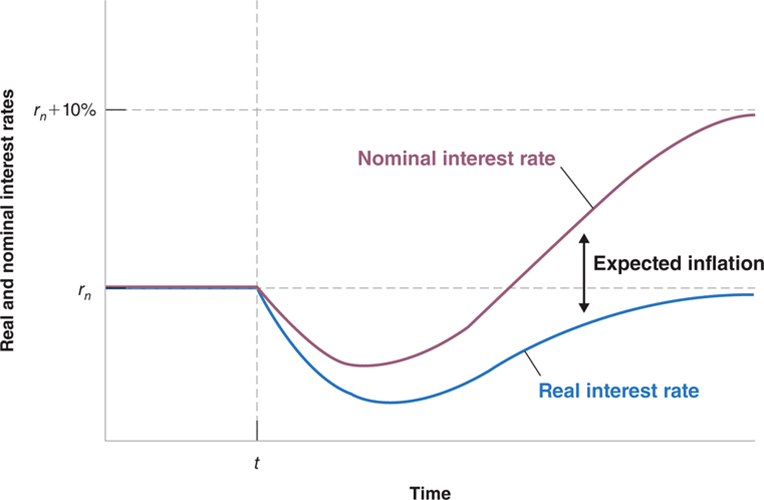
\includegraphics[scale=0.5]{graphs/L9F5.png}}
\end{column}
\end{columns}
\end{frame}

\begin{frame}{Nominal Interest Rates and Inflation Across Latin America}
\makebox[\linewidth][c]{
  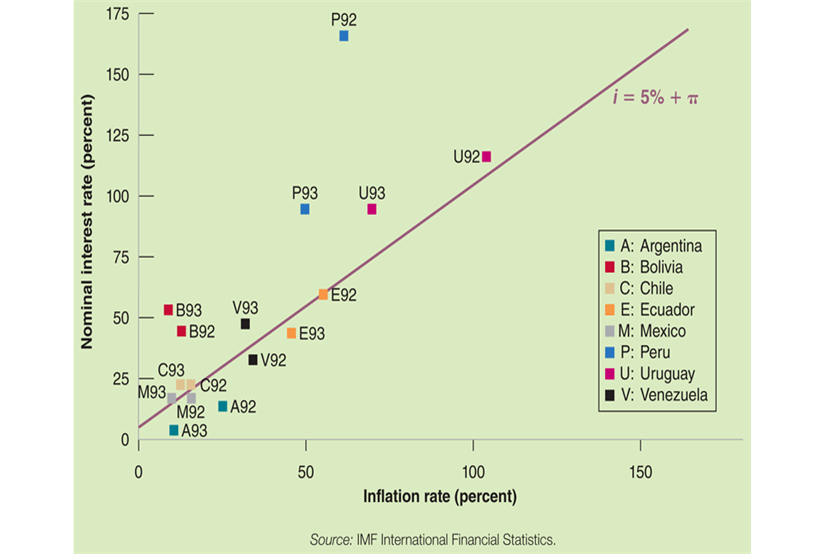
\includegraphics[scale=0.5]{graphs/L9F6.png}}
\end{frame}

\begin{frame}{Expected Present Discounted Value}
\begin{itemize}
\item Let interest rate be $i$ and investment be \rupee 1.
\item Discount factor: $\frac{1}{(1 + i)}$.
\pause
\item The present discounted value in today's rupees $V_t$
   \[ V_t = z_t + \frac{1}{(1 + i)}z_{t+1} + \frac{1}{(1 + i)^2}z_{t+2} + ... \]
\pause
\item Example: Let $i = 0.1$, the weight on payment 20 years later will be \pause 0.148. 
\item So, a payment of \rupee1000 in 20 years will be worth \rupee148.6 today.
\end{itemize}
\end{frame}

\begin{frame}{Expected Present Discounted Value}
A typical mortgage requires constant payment over a fixed time period.
\begin{itemize}
\item The present discounted value in today's rupees $V_t$
   \begin{equation*}
    V_t = z\bigg[ 1 + \frac{1}{(1 + i)} + \frac{1}{(1 + i)^2} + ... \bigg]
    \end{equation*}
\pause
\item The above is a sum of a GP.
     \begin{equation*}
     V_t = z\frac{1 - [1/(1 + i)^n]}{1 - [1/(1 + i)]}
     \end{equation*}
\item Example: interest rate = 5\%, annual payment = \rupee10,000, time = 20 years.
\end{itemize}
\end{frame}

\begin{frame}{Expected Present Discounted Value}
\textbf{Constant Interest Rate and Payment Forever}
\begin{itemize}
\item The present value would be
     \[ V_t = \frac{z}{i} \]
\item Example: $i = 5\%$, $z = 100$.
\end{itemize}
\end{frame}

\section{Chapter 15}
\begin{frame}{Bond Prices and Bond Yields}
Bonds vary across two variables: 
\begin{itemize}
\item[1] \textbf{Default Risk}
\item[2] \textbf{Maturity}
\end{itemize}
\pause
Let's focus on maturity.
\begin{itemize}
\item \textbf{Yield:} \pause The interest rate associated with the bond.
\item Yield and maturity are tied together. We call it the \textbf{term structure of interest rates}.
\pause
\item Let's think about 
     \begin{itemize}
     \item[1] \textit{Bond prices}
     \item[2] Examine the determinants of the yield curve.
     \item[3] The relationship between short-term and long-term interest rates.
     \end{itemize}
\end{itemize}
\end{frame}

\begin{frame}{Bond Prices and Present Value}
Two bonds: one-year and two-years.
\begin{itemize}
\item The price of one-year bond is 
     \[ P_{1t} = \frac{100}{1 + i_{1t}} \]
\item The price of two-years bond is 
     \[ P_{2t} = \frac{100}{(1 + i_{1t})(1 + i_{2t})} \]
\end{itemize}
NOTE: Interest rate is nominal one.
\end{frame}

\begin{frame}{Arbitrage and Bond Prices}
\begin{itemize}
\item Assumption: Investors care about \textbf{expected returns}.
\item Consequence: The two bonds must offer the same expected one-year returns.
\pause
\item If the above doesn't hold true, market for one bond will vanish. 
\pause
\item Arbitrage between the two bonds implies that the price of two years bond is the present value of the payment in two years.
\[ P_{2t} = \frac{100}{(1 + i_{1t})(1 + i_{1t + 1}^e)} \]
\end{itemize}
\end{frame}

\begin{frame}{Bond Prices and Bond Yields}
\begin{itemize}
\item \textbf{Yield to Maturity}: Constant interest rate that makes bond price equal to the present value of future payments on the bond. \pause
\item \[ P_{2t} = \frac{100}{(1 + i_{2t})^2} \] \pause
\item Some maths later: \[ i_{2t} = \frac{1}{2}(i_{1t} + i_{1t+1}^e) \]
\textit{The two year interest rate is the average of the current one year interest rate and next year's expected one-year interest rate.}
\end{itemize}
\end{frame}

\begin{frame}{The Yield Curve}
\begin{itemize}
\item Rearrange the interest rate equation to get
     \[ i^e_{1t + 1} = 2i_{2t} - i_{1t} \]
\item Let one year interest rate be 4\% and two-year rate be 5\%.
\item The interest rate in one year's time are supposed to be up by 6\%.
\end{itemize}
\end{frame}

\begin{frame}{Expectations Versus Reality: US Circa 2001}
\begin{columns}[T] % align columns
\begin{column}{.46\textwidth}
\begin{center}
\makebox[\linewidth][c]{
  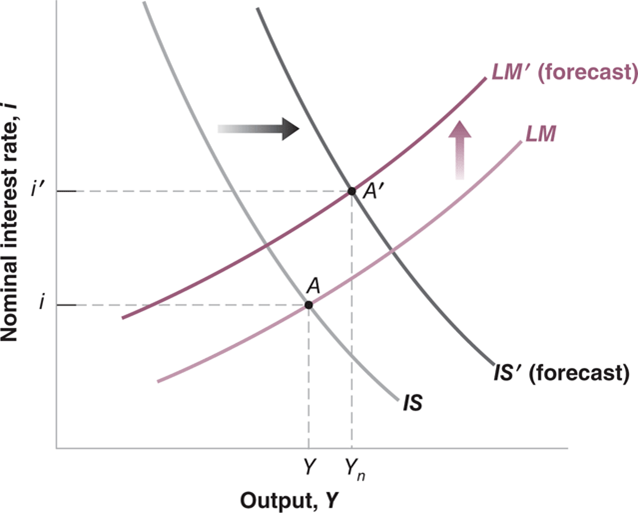
\includegraphics[scale=0.5]{graphs/L08F01.png}}
  %\caption{Expectations}
\end{center}
\end{column}
\hfill
\pause
\begin{column}{.46\textwidth}
\begin{center}
\makebox[\linewidth][c]{
  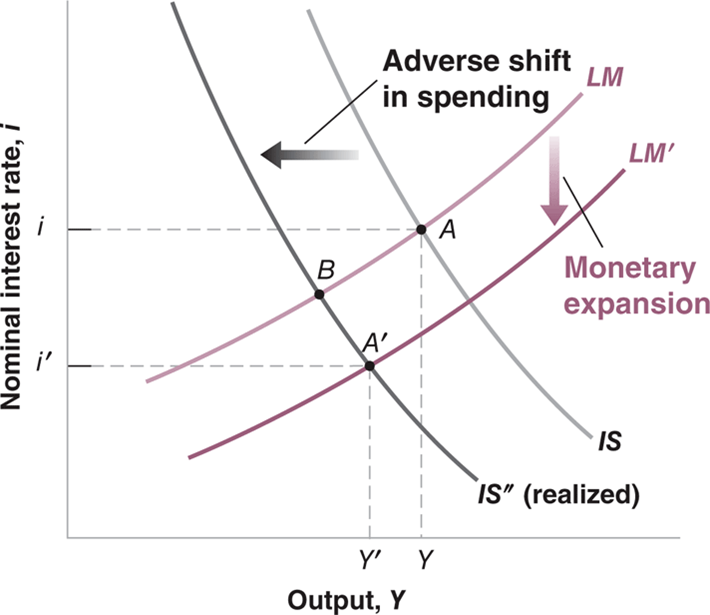
\includegraphics[scale=0.5]{graphs/L08F02.png}}
  %\caption{Reality}
\end{center}
\end{column}
\end{columns}
\pause
Try explaining the difference.
\end{frame}

\begin{frame}
\begin{center}
\makebox[\linewidth][c]{
  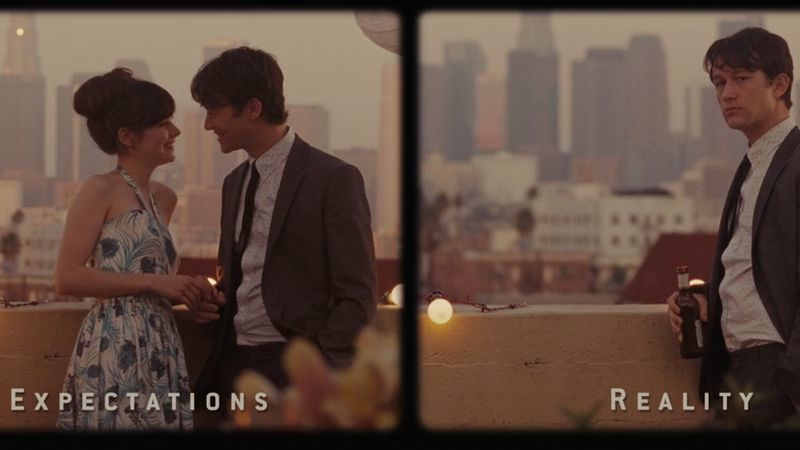
\includegraphics{graphs/L9ER.jpg}}
  %\caption{Reality}
\end{center}
\end{frame}

\begin{frame}{Stock Prices and Stock Market}
\begin{itemize}
\item Stock markets act as one source of firm finance.
\pause
\item Stocks pay dividends in an amount decided by the firm.
\pause
\item How do stock prices respond to macro-policy?
\pause
\item The real stock price is the present value of future dividends, discounted by interest rates.
\pause
\item $\uparrow$\texttt{Future dividends} $\Rightarrow$ $\uparrow$\texttt{real stock price}.
\item $\uparrow$\texttt{Future expected real interest rates} $\Rightarrow$ $\downarrow$\texttt{real stock prices}.
\end{itemize}
\end{frame}

\begin{frame}{Stock Market and Monetary Policy}
\begin{columns}[T] % align columns
\begin{column}{.36\textwidth}
\begin{itemize}
\item Let there be an unexpected monetary expansion.
\item Lower interest rate, and higher output (higher dividends).
\item A rise in stock prices.
\end{itemize}
\end{column}
\hfill
\pause
\begin{column}{.54\textwidth}
\makebox[\linewidth][c]{
  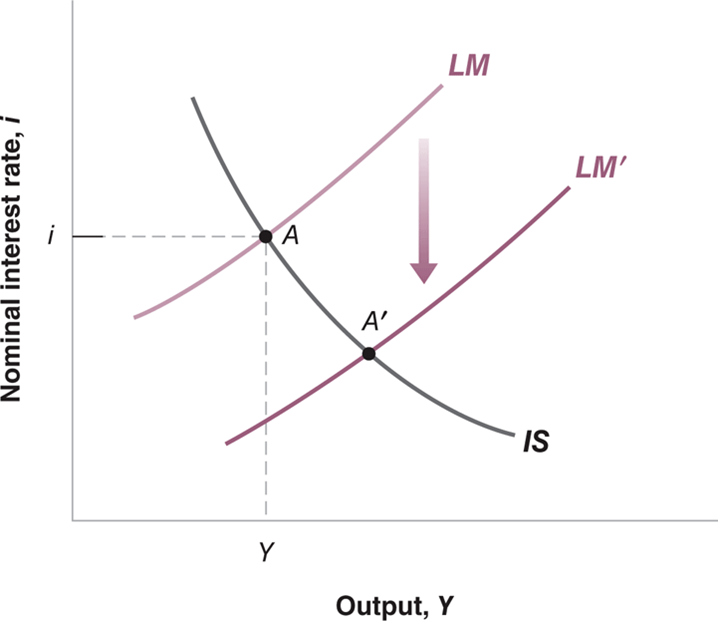
\includegraphics[scale=0.5]{graphs/L9F14.png}}
\end{column}
\end{columns}
\end{frame}

\begin{frame}{Stock Market and Consumer Spending}
\begin{columns}[T] % align columns
\begin{column}{.36\textwidth}
\begin{itemize}
\item Let there be rise in consumer spending.
\item Higher output (higher dividends).
\item A rise in stock prices.
\pause
\item \textcolor{red}{Incomplete story}. 
\end{itemize}
\end{column}
\hfill
\pause
\begin{column}{.54\textwidth}
\makebox[\linewidth][c]{
  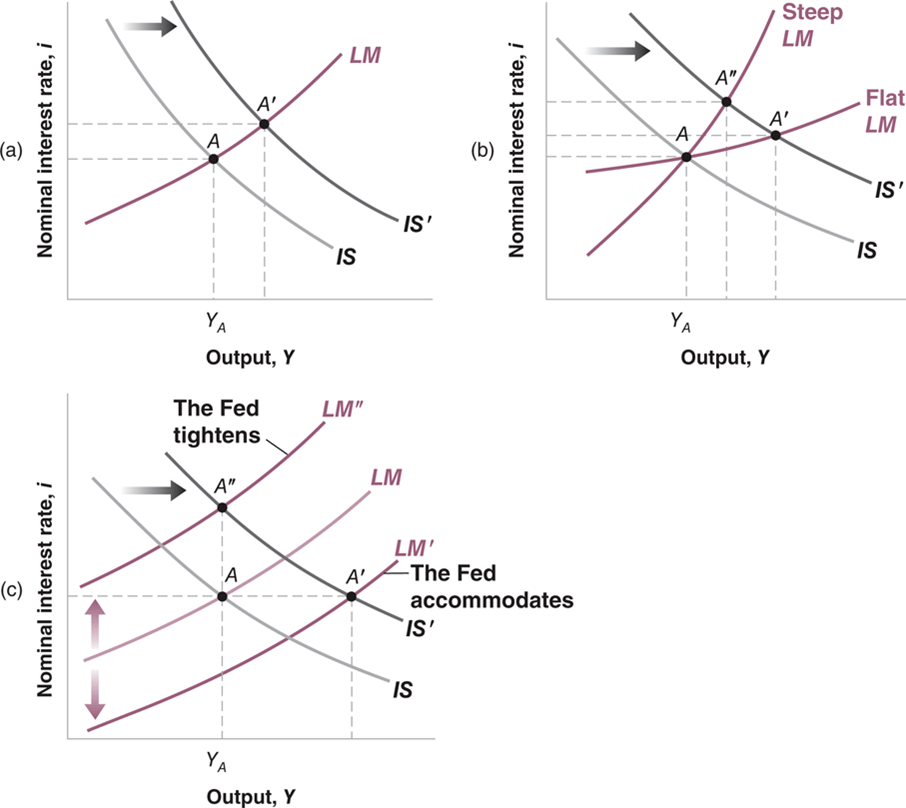
\includegraphics[scale=0.5]{graphs/L9F15.png}}
\end{column}
\end{columns}
\end{frame}

\begin{frame}{Risks, Bubbles, Fads}
\begin{itemize}
\item In 1994 a Russian ``financier'' Sergei Mavrodi, created a company called MMM and proceeded to sell shares, promising shareholders a rate of return of at least 3,000\% per year.
\item This was an instant hit.
\item  The price of MMM shares increased from 1,600 rubles (then worth \$1) to in February to 105,000 rubles (then worth \$51) in July.
\item The number of ``shareholders'' in July: millions.
\item The company wasn't involved in any real activity. 
\pause
\item The guy who ran this scam later ran for Parliament....\pause and won!
\end{itemize}
\end{frame}

\begin{frame}{Risks, Bubbles, Fads}
Three distinctive features of markets may give rise to bubbles:
\begin{itemize}
\item[1] \textit{Resale value}: A person may buy a house both for the rental income and also to make gains by holding on to the house and reselling it later.
\item[2] \textit{Ease of trading}:  You can switch between being a buyer and being a seller.
\item[3] \textit{Ease of borrowing to finance purchases}: If market participants can borrow to increase their demand for an asset that they believe will increase in price, well, we are staring at a possible bubble.
\end{itemize}
\end{frame}

\begin{frame}{Risks, Bubbles, and Fads}
\makebox[\linewidth][c]{
  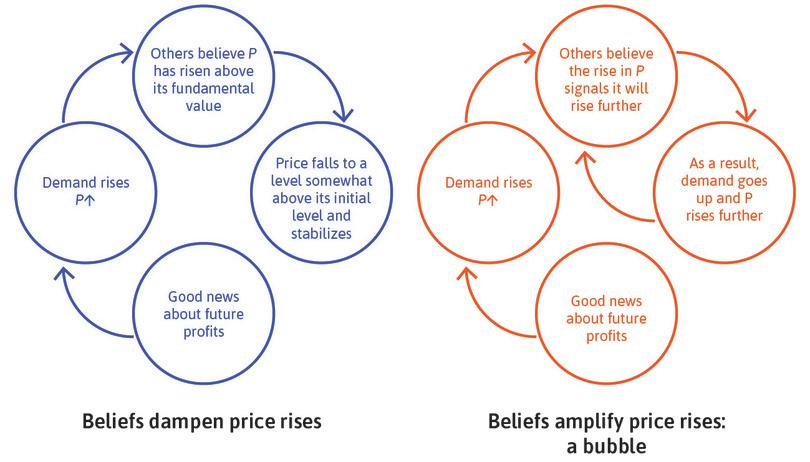
\includegraphics[scale=0.5]{graphs/L9F16.jpg}}
\end{frame}

\section{Chapter 16}

\begin{frame}{Agenda}
\begin{itemize}
\item Embed expectations into consumption decision.
\item Show that investments are function of expected interest rate.
\end{itemize}
\end{frame}

\begin{frame}{Consumption}
Consumption decision can take the following forms: 
\begin{itemize}
\item $C_t = C(\text{total wealth}_t)$.
\item $C_t = C(\text{total wealth}_t, Y_{Lt} - T_t)$.
\end{itemize}
\pause
Expectations impact consumption in two ways:
\begin{itemize}
\item[1] In order to compute future wealth, people form expectations about taxation, interest rate, etc.
\item[2] Stocks, bonds, and housing affect consumption indirectly.
\end{itemize}
\pause
\vspace{2mm}
Implications:
\begin{itemize}
\item[1] There may not be a one-to-one correspondence in current income and consumption movements.
\item[2] Consumption may rise even when there is no change in current income.
\end{itemize}
\end{frame}

\begin{frame}{A Model of Consumption}
\begin{itemize}
\item People like to consumption smooth
\item Let initial wealth = $W$, $R$ be number of working years, $Y_{Lt} - T_t$ is the annual income.
\item Let there be $L$ years in life.
\item $C = \frac{W + R(Y_{Lt} - T_t)}{L}$
\pause
\item $APC = \frac{C}{Y}$
\pause
\item In short run, average propensity to consume falls when income rises.
\item In long run, average propensity to consume doesn't change when income increases.
\end{itemize}
\end{frame}

\begin{frame}{Investment}
\begin{itemize}
\item Investments depend upon on the expected present value of future profits per unit capital.
\pause 
\item Present value of expected profits
     \[ V(\Pi_{t}^e) = \frac{1}{1 + r_t}\Pi_{t+1}^e + \frac{1}{(1 + r_{t})(1 + r_{t+1}^e)}(1 - \delta)\Pi_{t+2}^e \]
\pause
\item We can simplify the above equation by assuming future profits and interest rates to be same:
\pause
\item Under this assumption:
      \[ V(\Pi_t^e) = \frac{\Pi_t}{r + \delta} \]
\end{itemize}
\end{frame}

\begin{frame}{Investment}
\begin{itemize}
\item Investment can be written as 
     \[ I_t = I\Bigg(\frac{\Pi_t}{r + \delta}\Bigg) \]
\pause
\item $r + \delta$: user cost or the rental cost of capital.
\pause
\item $\Pi_t = \Pi\Bigg(\frac{Y_t}{K_t}\Bigg)$
\end{itemize}
\end{frame}

\begin{frame}{Investment and the Stock Market}
\begin{itemize}
\item Stock prices reflect incentives to invest
      \begin{itemize} 
      \item $\uparrow$ prices $\Rightarrow$ $\uparrow$ investment
      \item $\downarrow$ prices $\Rightarrow$ $\downarrow$ investment
      \end{itemize}
\pause
\item Tobin's $q$: \[ q = \frac{\text{Market Value of capital}}{\text{Replacement value of capital}} \]
\item In English: $q$ is basically the ratio of market to book value.
\pause
\item If $q < 1$, then \textcolor{red}{don't invest}.
\item If $q > 1$, then \textcolor{ao(english)}{invest}.
\end{itemize}
\end{frame}

\section{Chapter 17}
\begin{frame}{Agenda}
\begin{itemize}
\item Bring expectation effects into $IS-LM$.
\item Discuss monetary and fiscal policies.
\item Material: Blanchard, Chapter 17.
\end{itemize}
\end{frame}

\begin{frame}{Expectations and the $IS$ Relation}
\begin{itemize}
\item We define aggregate private spending as: 
    \[ A(Y, T, r) = C(Y-T) + I(Y,r) \]
\pause
\item Output now depends upon current and expected future parameters
    \[ Y = A(Y, T, r, Y^e, T^e, r^e) + G \]
\end{itemize}
\end{frame}

\begin{frame}{Expectations and the $IS$ Curve}
\begin{columns}[T] % align columns
\begin{column}{.52\textwidth}
  \begin{wideitemize}
    \item A fall in current interest rate does not have much impact on spending.
         \begin{itemize}
         \item A fall in current interest rate doesn't shift the present value.
         \item Firms are not likely to change their investment plans until the expectations shift.
         \end{itemize}
    \item The multiplier is going to be smaller. 
     \end{wideitemize}
\end{column}%
\pause
\hfill%
\begin{column}{.44\textwidth}
  \makebox[\linewidth][c]{
    \resizebox{\linewidth}{!}{
      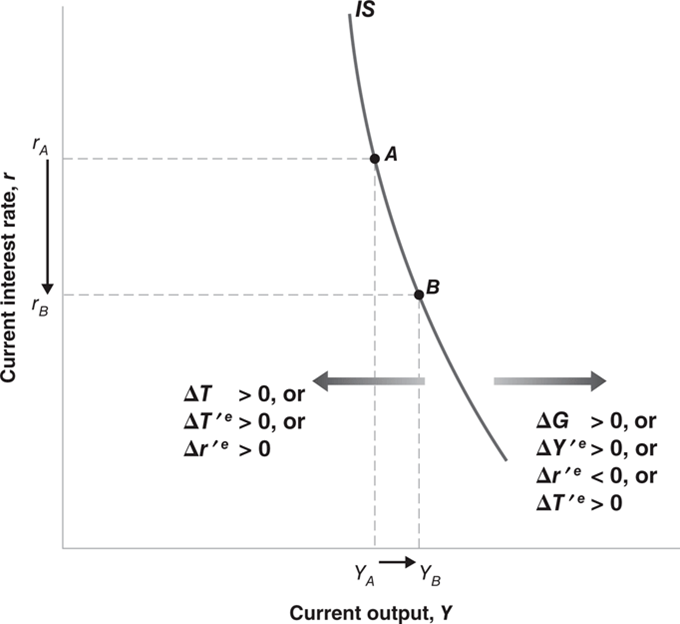
\includegraphics{graphs/L9F17.png}
    }
  }
\end{column}%
\end{columns}
\end{frame}

\begin{frame}{The $LM$ Curve Revisited}
\begin{wideitemize}
    \item Decision to hold money is a myopic one.
         \begin{itemize}
         \item Depends upon current income and current interest rate.
         \item Doesn't depend upon future expected nominal interest rate.
         \end{itemize}
    \item The multiplier is going to be smaller. 
\end{wideitemize}
\end{frame}

\begin{frame}{Expectations and the $IS$ Curve}
\begin{columns}[T] % align columns
\begin{column}{.52\textwidth}
  \begin{wideitemize}
   \item $IS$: \begin{equation*}
            Y = A(Y, T, r, Y^e, T^e, r^e) + G
               \end{equation*}
   \item $LM$: \begin{equation*}
           \frac{M}{P} = YL(r)  
               \end{equation*}     
   \end{wideitemize}
\end{column}%
\pause
\hfill%
\begin{column}{.44\textwidth}
  \makebox[\linewidth][c]{
    \resizebox{\linewidth}{!}{
      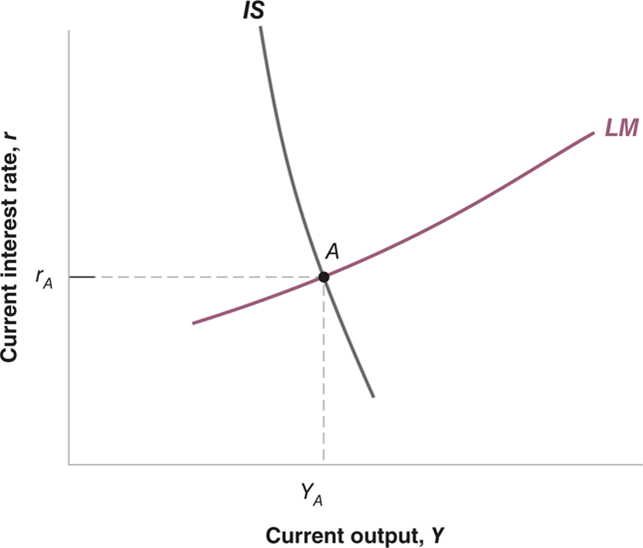
\includegraphics{graphs/L9F18.png}
    }
  }
\end{column}%
\end{columns}
\end{frame}

\begin{frame}{Monetary Policy Revisited}
\begin{columns}[T] % align columns
\begin{column}{.52\textwidth}
  \begin{wideitemize}
   \item Money supply goes up $\Rightarrow$ Output shift may be larger. Why?
   \pause
   \item The answer depends upon what firms and consumers expect.     
   \pause
   \item These expectations are NOT random. 
   \end{wideitemize}
\end{column}%
\pause
\hfill%
\begin{column}{.44\textwidth}
  \makebox[\linewidth][c]{
    \resizebox{\linewidth}{!}{
      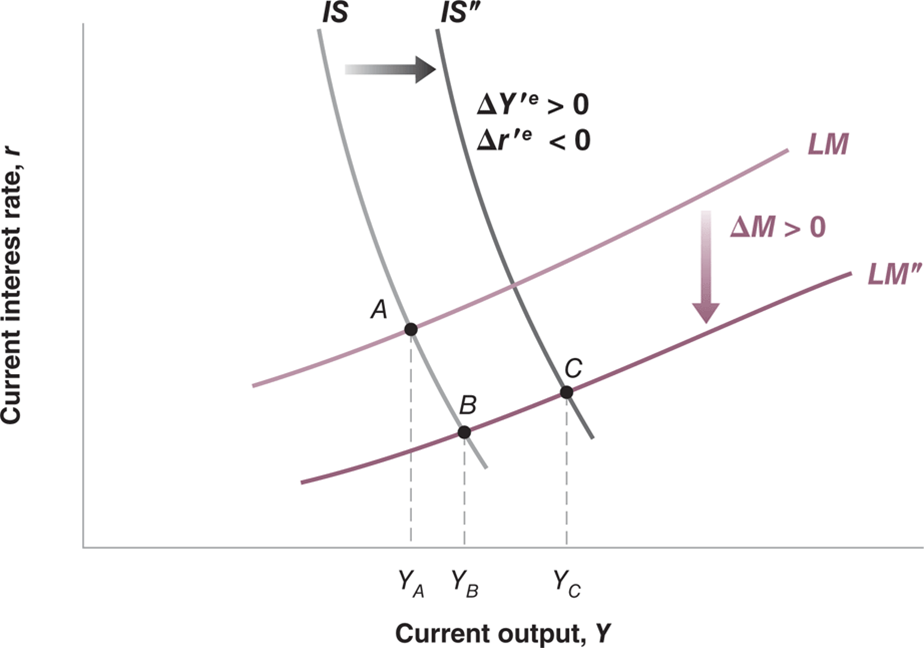
\includegraphics{graphs/L9F19.png}
    }
  }
\end{column}%
\end{columns}
\end{frame}

\begin{frame}{The Liquidity Trap, QE, and Expectations}
Three channels through which QE may affect the economy.
\begin{itemize}
\item[1] Arbitrage may not hold. By buying assets, the central bank can replace risk-averse investors.
          \begin{itemize}
          \item The price of the asset rise (interest rate falls).
          \item The central bank may even finance some of the borrowers
          \end{itemize}
\pause
\item[2] Expectations of future nominal interest rates. 
         \begin{itemize}
         \item If expansionary monetary policy signals future expansionary policies, signal may be +ve.
         \item Future nominal rates go up $\Rightarrow$ Spending goes up.
         \end{itemize}
\pause
\item[3] Expectations of inflation.
         \begin{itemize}
         \item Higher expected inflation $\Rightarrow$ $\downarrow$ current (and future) expected real interest rates.
         \end{itemize}
\end{itemize}
\end{frame}

\begin{frame}{Deficit Reduction Redux}
\begin{columns}[T] % align columns
\begin{column}{.52\textwidth}
  \begin{wideitemize}
   \item Lower public spending means higher private spending. (Spending = Public + Private)
   \pause
   \item Higher private spending requires lower interest rates.     
   \pause
   \item The expected future interest rate goes down, stimulating spending and increasing output.
   \end{wideitemize}
\end{column}%
\pause
\hfill%
\begin{column}{.44\textwidth}
  \makebox[\linewidth][c]{
    \resizebox{\linewidth}{!}{
      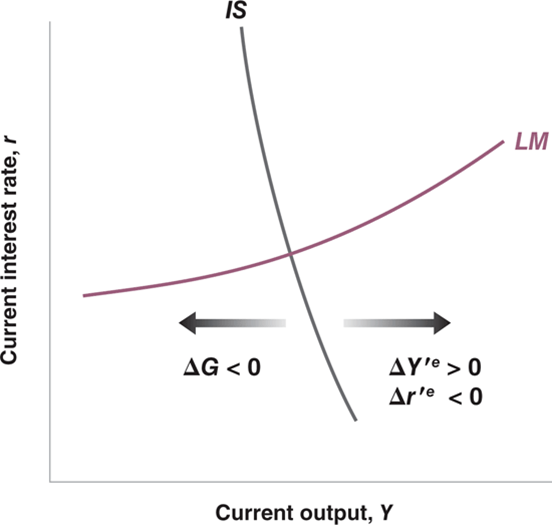
\includegraphics{graphs/L9F20.png}
    }
  }
\end{column}%
\end{columns}
\end{frame}


\end{document}
